\chapter{Deep Neural Networks}
\label{chapter:cnn}
%PAPERS TO USE FOR CITING
%https://ieeexplore.ieee.org/abstract/document/6639344
%http://papers.nips.cc/paper/4824-imagenet-classification-with-deep-convolutional-neural-networ



\quad A Neural Network (NN) is an interconnected group of nodes that follow a computational model that propagates data forward while processing. 
The earliest Neural Networks were proposed by McCulloh and Pitts~\cite{neuron:model}
, in which a Neuron has a linear part, based on aggregation of data and then a non linear part called the activation function. The issue with using only one neuron
is that it isn't able to be used in non-linear separable problems.
By aggregating several neurons in layers and the input of each neuron as in figure~\ref{MLP}
being based on the previous layers, that problem can be eliminated.

\begin{figure}[!htbp]
    \centering
    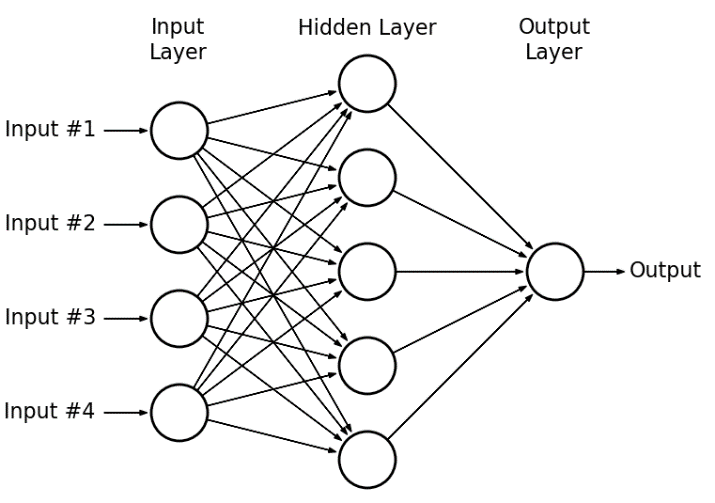
\includegraphics[width=0.7\textwidth]{Figures/mlp-tobereplaced.png}
    \caption{Multi Layer Perceptron- IMAGE TO BE REPLACED}
    \label{MLP}
\end{figure} 


 Each input to a Neuron contributes differently to the output. This share is dependent on the weight value. 
 These are obtained by training the network through various techniques, one of which is Deep Supervised
 Learning~\cite{deeplearning}
 . For a certain input, there's an expected output and the real output of the NN. Then the loss function based on these outputs
 is calculated and then the weight values are iteratively modified for better outputs by the Neural Network.



 A Deep Neural Network (DNN) is a NN that uses this approach for learning. It has multiple hidden layers and it can 
 model complex non-linear relationships. If the activation function isn't a polynomial, it satisfies
 the Universal approximation problem~\cite{approximation:problem}.

One of the limitations of traditional Networks is the complexity that is given between each layer. Let's use the example of hand digit recognition problem.
The MNIST data set is composed of 28x28 grayscaled images~\cite{mnist:digits}. In a traditional fully connected Neural Network, a neuron from the second layer
would have 28x28 weights. That's 3.136 kiloBytes per neuron of weight values while using Floating-Point 32 bit (FP32). 
By making the layer size constant, the computational power required grows exponentially.
When building a more complex network for image recognition, the input layer grows and so by default does the number of weights.


%One propriety of CNN's is the shift invariance due to the use of 2D image convolution with filters and that makes them specifically
%good for Image and video recognition.

 \section{Convolutional Neural Networks}
 \label{section:subcnn}

 \quad Convolutional Neural Networks (CNN) are a class of DNNs used in Image and Video recognition due to their shift invariance characteristic. They were first proposed in the 
 1980's but it wasn't until 2012 with AlexNet~\cite{alexnet} 
 that CNNs really took off. Fundamentally,  it's a regularized version of Multilayer Perceptrons (MLP).

 These networks fix the issues discussed due to each neuron of the following layer being connected to a few of the previous layer.
 

 \begin{figure}[!htbp]
    \centering
    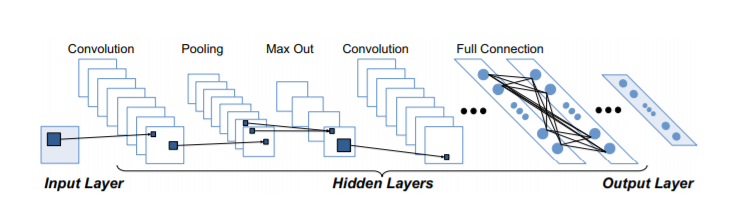
\includegraphics[width=0.7\textwidth]{Figures/convolutionlayer.png}
    \caption{CNN- IMAGE TO BE REPLACED}
    \label{CNNl}
\end{figure} 

 \subsection{Architecture Overview}
 \label{section:Aoverview}


 %There's several types of layers used in these networks to achieve the desired result.

 \subsubsection{Convolutional Layer}
\label{section:convlayer}

\quad The most processing time consuming  is the Convolutional Layer due to it's raw processing needs. 
It takes an input with several dimensions: image width,height and color space for the first layer,
for the following convolutional layers it takes a 3D array: map width,height and number of channels.
For the earlier example of the MNIST
data set, it would be 28x28x1 as it's a 2D image in grayscale.

To compute a neuron in the next layer we get the convolution in equation~\ref{equation:convolution} and image representation in figure \ref{Cl},
where $x_{j}^{l+1}$ is the output, $\delta$ is the activation function, which depends on the architecture, $x_{i}^{l}$ is the input of the convolution layer, $k_{ij}^{l+1}$ is
the kernel of said layer which is obtained by training the network and $b_{j}^{l+1}$ is the bias.
\begin{equation} \label{equation:convolution}
   %\resizebox{.5 \textwidth}{!} 
    %%
\end{equation}

Thus an output neuron depends only on a small region of the input which is called the local receptive field. 

\begin{figure}[!htbp]
    \centering
    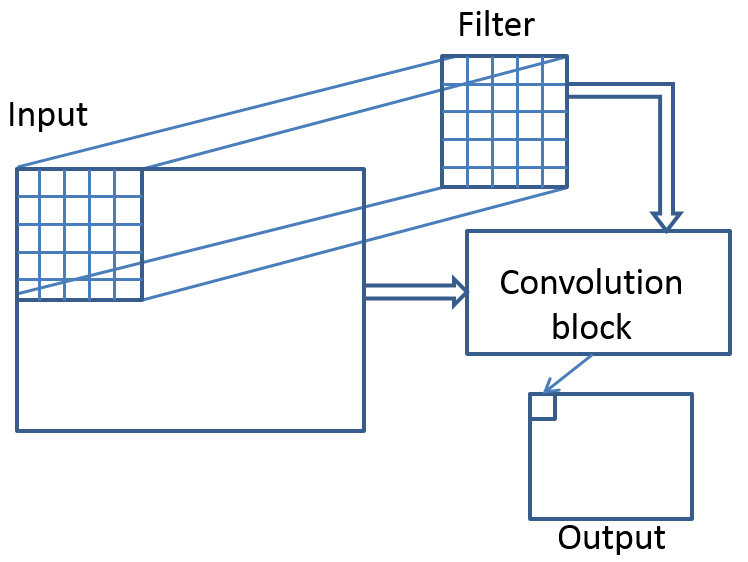
\includegraphics[width=0.5\textwidth]{Figures/convolution.png}
    \caption{2D CONV- TO BE REPLACED}
    \label{Cl}
\end{figure} 

The output's dimensions depend on several parameters of the convolution such as zero-padding and stride. The Former means to add 0's around the edges
of the input matrix. The latter means the step used for the convolution, if the value is e.g 2, it will skip a pixel each iteration of the convolution.
The equation in~\ref{equation:padding} can be used to calculate the output size. Where $n$ is the width/height of the input of layer $l$,
$ b$ is the width/height of the kernel, $p$ is  zero-padding while $s$ is the stride.

\begin{equation} \label{equation:padding}
     n^{l+1} = \frac{n^{l}- b^{l}+2 \times p}{s}
\end{equation}

The number of channels of the output is equal to the number of filters
in the convolutional layer.



%Then a 3D convolution is performed with the kernel changing from layer to layer

\subsubsection{Pooling Layer}

\quad The MaxPool or AvgPool are layers used in Convolutional Neural Networks to downsampling the feature maps to make 
the output maps less sensitive to the location of the features.

Maximum Pooling or MaxPool, like it's suggested in it's name groups $ n * n $ points and outputs the pixel with highest value.
 The output will have it's size lowered by $ n $ times.
The Average Pooling or AvgPool, instead takes all of the input points and calculates the average. Downsampling can also be achieved by using convolutions with stride 2 and padding equal to 1.
Upsample layers can be also used that turn each pixel into $ n^{2} $, where n is the amount of times the output will be bigger than the input.

\begin{figure}[!htbp]
    \centering
    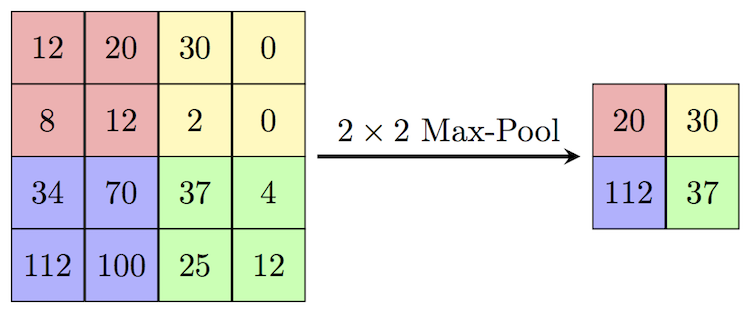
\includegraphics[width=0.5\textwidth]{Figures/maxpool.png}
    \caption{MAXPOOL- TO BE REPLACED}
    \label{figure:maxpool}
\end{figure} 
 

\subsubsection{Fully Connected Layer}

\quad The fully Connected Layer is mostly used for classification in the final layers of the Neural Network. It associates the feature map to the respective labels.
It takes the 3D vector and outputs a single vector thus it's also known as flatten.
 The equation in~\ref{equation:connected} describes the operation. Here $w_{ji}^{l+1}$ are the weights
 associated with a specific input for each output pixel.



\begin{equation} \label{equation:connected}
    %\resizebox{.5 \textwidth}{!} 
     %%
 \end{equation}
 


\subsubsection{Route $\&$ Shortcut Layer}

\quad The Shortcut layer or skip connection was first introduced in Resnet \cite{resnet}.
It allows to connect the previous layer to another to allow the flow of information across layers.
The Route layer, used in Yolov3~\cite{yolov3}
,concatenates 2 layers in depth (channel) or skips the layer forward. This is used after the detection layer in Yolov3 to extract other features.

\subsubsection{Dropout Layer}

\quad This type of layer was conceived to avoid overfitting \cite{Dropout}
by dropping the neurons with probability below the threshold. In figure \ref{figure:Dropout}, there's a
graphical representation.
\begin{figure}[!htbp]
    \centering
    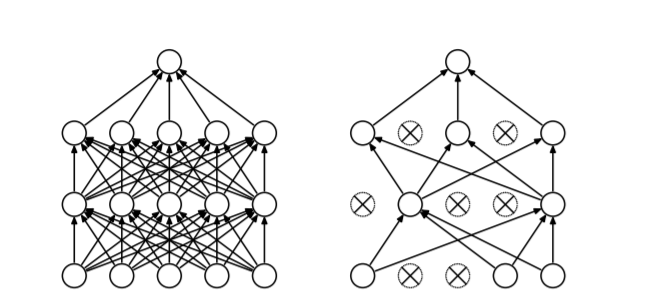
\includegraphics[width=0.6\textwidth]{Figures/dropout.png}
    \caption{Dropout if applied to all layers, adapted from~\cite{Dropout}}
    \label{figure:Dropout}
\end{figure} 

\subsubsection{Activation Functions}

\quad Activation Functions (AF) are functions used in each layer of a Neural Network to compute the weighted sum of input and biases,
which is used to give a value to a neuron.Non-linear AFs are used to transform linear inputs to non-linear outputs.
 While training Deep Neural Networks, vanishing and exploding gradients
are common issues, in other words, after successive multiplications of the loss gradient, the values tend to tend to 0 or infinity and thus the gradient disappears.
AFs help mitigate this issue by keeping the gradient in specific limits. The most popular activation functions can be found in table~\ref{table:AF}.



\begin{table}[]
    \centering
    \resizebox{.6\textwidth}{!}{%}
    \begin{tabular}{ll}
    \hline
    \textbf{Activation Functions} & \textbf{Computation Equation} \\ \hline \hline
    Sigmoid                       &  $\displaystyle f(x)=\frac{1}{1+ e^{-x}}$                             \\ \hline
    Tanh                          &  $\displaystyle f(x)=\frac{e^{x}-e^{-x}}{e^{x}+e^{-x}}$                            \\ \hline
    Softmax                       &  $\displaystyle f(x_{i})=\frac{x_{i}}{\sum_{j}e^{x_{j}}}$                             \\ \hline
    ReLU                          &    $ f(x)=\begin{matrix}
        x & if & x\geq 0  \\ 
        0 & if & x< 0 
    \end{matrix} $                           \\ \hline
    LReLU                         &  $f(x)= \begin{matrix}
        x & if & x > 0  \\ 
        \alpha x & if & x \leq 0 
    \end{matrix} $                        \\ \hline
    ELU                           &             $ f(x)=\begin{matrix}
        x & if & x> 0  \\ 
        \alpha e^{x} - 1 & if & x\leq 0 
    \end{matrix} $                 \\ \hline
    \end{tabular}%
    }
    \caption{Popular Activation functions}
    \label{table:AF}
\end{table}


%image of activation functions?

 \section{Frameworks for Neural Networks}
 \label{section:darknet}

\quad To run a Neural Network model there's several popular frameworks like Tensorflow, PyTorch, Caffe and Darknet.
Their propose is to offer abstraction to software developers that want to run these networks. They also offer
programming for different platforms like nVidia GPU's by using the CUDA API.


\subsection{Darknet}

\quad Darknet~\cite{darknet} is an open source neural network framework written in C and CUDA.It's used as the backbone for Yolov3~\cite{yolov3} and supports several different network configurations such as AlexNet and Resnet.
 It utilizes a network configuration
file (.cfg) and a weights file (.weights) as input for inference.

\lstinputlisting[label=cfg,language=Python,frame=single,breaklines=true,firstline=13,lastline=19,caption=cfg code for a Convolutional Layer used in Yolov3~\cite{yolov3}]{./Code/yolov3.cfg}

In listing \ref{cfg}, there's a snippet of the file featuring
a convolution layer with 32 kernels of size 3x3. It has stride of 1 and zero padding of 1, meaning the output size will
be equal to the input. The input size can be calculated by analyzing the previous layers and the network parameters. The network parameters in \ref{net} includes
data to be used for training while only the first three parameters are needed for inference.

\lstinputlisting[label=net,language=Python,frame=single,breaklines=true,firstline=1,lastline=11,caption=cfg code for the network parameters]{./Code/yolov3.cfg}


\subsection{Caffe}


\quad Convolutional Architecture for Fast Feature Embedding (Caffe)~\cite{caffe} is also an Open source framework written in C++ with interface for Python.
Caffe exports a neural network by serializing it using the Google Protocol Buffers (ProtoBuf) serialization library. Each network has 2 prototxt files:
\begin{itemize}
    \item  deploy.prototxt- File that describes the structure of the network that can be deployed for inference.
    \item  train\_val.prototxt- File that includes structure for training. 
    it includes the extra layers used to aid the training and validation process.
\end{itemize}

The interface for python helps generate these files. For inference only the deploy file matters.

\lstinputlisting[label=caffe,language=Python,frame=single,breaklines=true,firstline=1,lastline=26,caption=prototxt file for the input data and the first convolution layer of AlexNet~\cite{alexnet}]{./Code/caffe.prototxt}
